\chapter{Integration into RTA-CAR Project}
\label{ch:IntGuide}

This chapter aims to provide a guideline for the integration of RTA-SUM SSFM module into an RTA-CAR project.

Once RTA-SUM plugin is installed, RTA-SUM SSFM gets available for being integrated into a project. Create a new RTA-CAR project in ISOLAR-AB and select the SDV 2.0 version. 
Open the RTA Code Generator dialog and enable RTA-SUM SSFM by choosing the SDV 2.0 selected during the project creation. If the option Not Configured is chosen instead, the module will not be integrated.

Refer to RTA-SUM plugin Getting Started Guide for further details.

\section {Prerequisites}
\begin{itemize}
\item It is assumed the integrator has followed the RTA-SUM Getting Started Guide to install the RTA-SUM plugin.
\item In order to successfully follow this guide, you shall have the RTA-CAR toolchain installed and you must be familiar with the AUTOSAR specifications, terminology and methodology. You also must be familiar with the GM specification and GM-SUM modules functionalities.
\end{itemize}

\section{Create SSFM module}

From the 'ECU Navigator' view, expand the Bsw Modules, and add the 'SSFM' module to the 'Other Modules', as shown below:

%\begin{figure}[H]
%	\centering
%	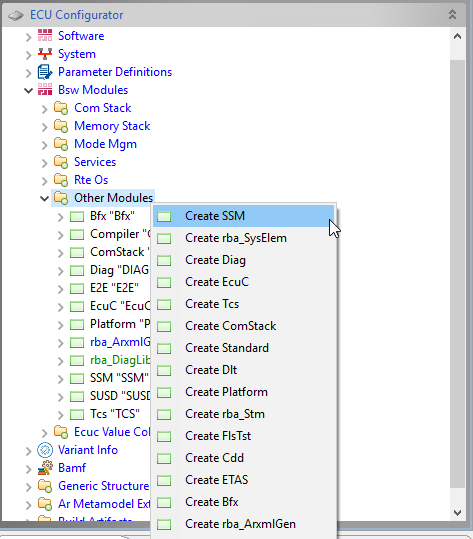
\includegraphics[scale=0.35]{images/createSSM.png}
%\end{figure}

\section{SSFM Configuration}
N/A

\section{MemMap Generation}
\label{sec:MemMap}

After generating the SUM files, execute the MemMap tool to generate memory mapping file of the module (\file{SUM\_SSFM\_MemMap.h}).